\documentclass[12pt]{../style-files/ociamthesis}
 
\usepackage{amssymb}
\usepackage{titlesec}
\usepackage{amsmath}
\usepackage{float}
\usepackage{graphicx}
\usepackage{caption}
\usepackage{subfig}
\usepackage{xcolor}
\usepackage[section]{placeins}
\usepackage{mathrsfs}
\usepackage{bm}
\usepackage{stmaryrd}
\usepackage{siunitx}
\usepackage{rotating}
\usepackage[utf8]{inputenc}
\usepackage[round]{natbib}
\usepackage{tikz}
\usetikzlibrary{fadings}
\usetikzlibrary{snakes}

\usepackage{geometry}
 \geometry{
 a4paper,
 left=40mm,
 right=30mm,
 top=30mm,
 bottom=30mm
 }

\definecolor{theblue}{HTML}{0000CD}

% disable this package for printed version
\usepackage[colorlinks=true, linktocpage=true, allcolors=theblue]{hyperref}

\titleformat{\chapter}[display]
  {\bfseries\Large}
  {\filright\MakeUppercase{\chaptertitlename} \Large\thechapter}
  {1ex}
  {}
  [\vspace{1ex} \hrule \vspace{1pt} \hrule]

\newcommand{\adv}{    {\it Adv. Space Res.}} 
\newcommand{\annG}{   {\it Ann. Geophys.}} 
\newcommand{\aap}{    {\it Astron. Astrophys.}}
\newcommand{\aaps}{   {\it Astron. Astrophys. Suppl.}}
\newcommand{\aapr}{   {\it Astron. Astrophys. Rev.}}
\newcommand{\ag}{     {\it Ann. Geophys.}}
\newcommand{\aj}{     {\it Astron. J.}} 
\newcommand{\apj}{    {\it Astrophys. J.}}
\newcommand{\apjl}{   {\it Astrophys. J. Lett.}}
\newcommand{\apss}{   {\it Astrophys. Space Sci.}} 
\newcommand{\cjaa}{   {\it Chin. J. Astron. Astrophys.}} 
\newcommand{\gafd}{   {\it Geophys. Astrophys. Fluid Dyn.}}
\newcommand{\grl}{    {\it Geophys. Res. Lett.}}
\newcommand{\ijga}{   {\it Int. J. Geomagn. Aeron.}}
\newcommand{\jastp}{  {\it J. Atmos. Solar-Terr. Phys.}} 
\newcommand{\jgr}{    {\it J. Geophys. Res.}}
\newcommand{\mnras}{  {\it Mon. Not. Roy. Astron. Soc.}}
\newcommand{\na}{     {\it New Astronomy}}
\newcommand{\nat}{    {\it Nature}}
\newcommand{\pasp}{   {\it Pub. Astron. Soc. Pac.}}
\newcommand{\pasj}{   {\it Pub. Astron. Soc. Japan}}
\newcommand{\pre}{    {\it Phys. Rev. E}}
\newcommand{\solphys}{{\it Solar Phys.}}
\newcommand{\sovast}{ {\it Soviet  Astron.}} 
\newcommand{\ssr}{    {\it Space Sci. Rev.}}
\newcommand{\caa}{    {\it Chinese Astron. Astrohpys.}} 
\newcommand{\apjs}{   {\it Astrophys. J. Suppl.}}

\begin{document}

\baselineskip=18pt

\setcounter{secnumdepth}{3}
\setcounter{tocdepth}{3}

\setcounter{chapter}{1}


\newcommand{\bv}{\mathbf{v}}
\newcommand{\bB}{\mathbf{B}}


%------------------------------------------------------------------------------
\chapter{Asymmetric waveguides - eigenvalue problem}
\label{chap: EVP}
%------------------------------------------------------------------------------

The simplest model of an asymmetric waveguide is an asymmetric magnetic slab in a non-magnetic environment\footnote{More precisely, the simplest model of an asymmetric MHD waveguide is an interface between different plasmas; the asymmetric slab is the simplest asymmetric waveguide that can oscillate in a collective body mode (see Section~\ref{sec: body}).}

%------------------------------------------------------------------------------
\section{Chapter introduction}
\label{sec: EVP intro}
%------------------------------------------------------------------------------

Section~\ref{sec: EVP non-mag} is based on \cite{all_etal17} and Section~\ref{sec: EVP mag} is based on \cite{zsa_etal18}.

%------------------------------------------------------------------------------
\section{Asymmetric slab}
\label{sec: asym slab}
%------------------------------------------------------------------------------
\subsection{Model description}
Figure~\ref{fig:eq} illustrates the construction of this mathematical model, where a three-dimensional, unbounded, inviscid plasma is separated into three regions by two parallel planar interfaces at $x = \pm x_0$. The magnetic field is in the $z$-direction and has magnitude
\begin{equation}
	B(x)=
	\begin{cases}
		B_1 & \text{if } x < -x_0, \\
		B_0 & \text{if } |x|\leq{x_0}, \\
		B_2 & \text{if } x > x_0,
	\end{cases}
\end{equation}
where $B_j$, for $j = 0, 1, 2$ are constant. Within each region, denoted by subscripts 0, 1, and 2, the plasma is uniform and the equilibrium plasma pressure, density, and temperature are denoted by $p_j$, $\rho_j$, and $T_j$, respectively, for $j = 0, 1, 2$.

\begin{figure}
	\centering
	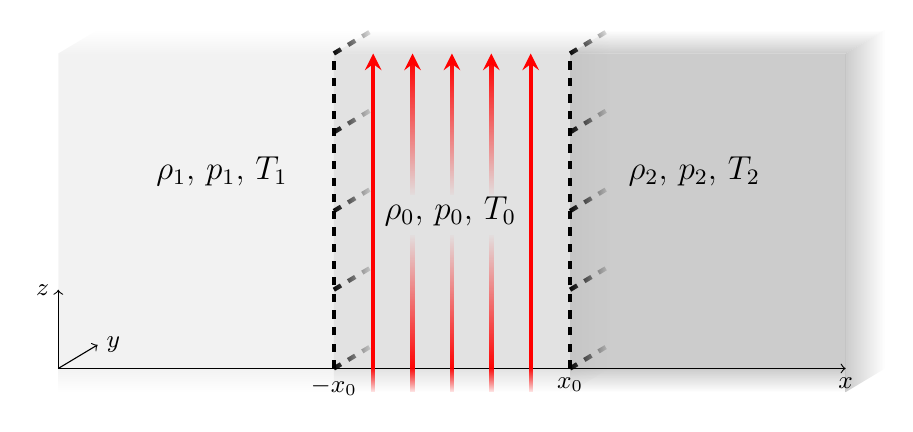
\begin{tikzpicture}
	\path [fill=lightgray, opacity=0.45] (3.5,0) -- (3.5,4) -- (6.5,4) -- (6.5,0) -- (3.5,0);
	\shade[left color=lightgray,right color=white, opacity=0.45] (6.5,0) -- (6.5,4) -- (7,4.3) -- (7,0.3) -- (6.5,0);
	\shade[top color=lightgray,bottom color=white, opacity=0.45] (3.5,0) -- (6.5,0) -- (6.5,-0.3) -- (3.5,-0.3) -- (3.5,0);
	\shade[top color=white,bottom color=lightgray, opacity=0.45] (3.5,4) -- (4,4.3) -- (7,4.3) -- (6.5,4) -- (3.5,4);
	\shade[left color=lightgray,right color=white, opacity=0.45] (6.5,0) -- (6.5,-0.3) -- (7,0) -- (7,0.3) -- (6.5,0);
	
	\path [fill=lightgray, opacity=0.8] (6.5,0) -- (6.5,4) -- (10,4) -- (10,0) -- (6.5,0);
	\shade[top color=lightgray,bottom color=white, opacity=0.8] (6.5,0) -- (10,0) -- (10,-0.3) -- (6.5,-0.3) -- (6.5,0);
	\shade[top color=white,bottom color=lightgray, opacity=0.8] (6.5,4) -- (7,4.3) -- (10.5,4.3) -- (10,4) -- (6.5,4);
	\shade[left color=lightgray,right color=white, opacity=0.8] (10,-0.3) -- (10,4) -- (10.5,4.3) -- (10.5,0) -- (10,-0.3);
	
	\path [fill=lightgray, opacity=0.2] (0,0) -- (0,4) -- (3.5,4) -- (3.5,0) -- (0,0);
	\shade[top color=lightgray,bottom color=white, opacity=0.2] (0,0) -- (3.5,0) -- (3.5,-0.3) -- (0,-0.3) -- (0,0);
	\shade[top color=white,bottom color=lightgray, opacity=0.2] (0,4) -- (0.5,4.3) -- (4,4.3) -- (3.5,4) -- (0,4);
	
	\draw [<->] (0,1) -- (0,0) -- (10,0);
	\draw [->] (0,0) -- (0.5,0.3);
	
	\draw [ultra thick, dashed] (3.5,0) -- (3.5,4);
	\draw [ultra thick, dashed, path fading=east] (3.5,0) -- (4,0.3);
	\draw [ultra thick, dashed, path fading=east] (3.5,4) -- (4,4.3);
	\draw [ultra thick, dashed, path fading=east] (3.5,2) -- (4,2.3);
	\draw [ultra thick, dashed, path fading=east] (3.5,1) -- (4,1.3);
	\draw [ultra thick, dashed, path fading=east] (3.5,3) -- (4,3.3);
	\draw [ultra thick, red, -stealth] (4,0) -- (4,4);
	\draw [ultra thick, red, path fading=south] (4,-0.3) -- (4,0);
	\draw [ultra thick, red, path fading=north] (4.5,0) -- (4.5, 1.7);
	\draw [ultra thick, red, path fading=south] (4.5,-0.3) -- (4.5,0);
	\draw [ultra thick, red, path fading=south] (4.5,2.2) -- (4.5,3.9);
	\draw [ultra thick, red, -stealth] (4.5,3.9) -- (4.5,4);
	\draw [ultra thick, red, path fading=north] (5,0) -- (5, 1.7);
	\draw [ultra thick, red, path fading=south] (5,-0.3) -- (5, 0);
	\draw [ultra thick, red, path fading=south] (5,2.2) -- (5,3.9);
	\draw [ultra thick, red, -stealth] (5,3.9) -- (5,4);
	\draw [ultra thick, red, path fading=north] (5.5,0) -- (5.5, 1.7);
	\draw [ultra thick, red, path fading=south] (5.5,-0.3) -- (5.5, 0);
	\draw [ultra thick, red, path fading=south] (5.5,2.2) -- (5.5,3.9);
	\draw [ultra thick, red, -stealth] (5.5,3.9) -- (5.5,4);
	\draw [ultra thick, red, -stealth] (6,0) -- (6,4);
	\draw [ultra thick, red, path fading=south] (6,-0.3) -- (6,0);
	\draw [ultra thick, dashed] (6.5,0) --(6.5,4);
	\draw [ultra thick, dashed, path fading=east] (6.5,0) -- (7,0.3);
	\draw [ultra thick, dashed, path fading=east] (6.5,4) -- (7,4.3);
	\draw [ultra thick, dashed, path fading=east] (6.5,2) -- (7,2.3);
	\draw [ultra thick, dashed, path fading=east] (6.5,1) -- (7,1.3);
	\draw [ultra thick, dashed, path fading=east] (6.5,3) -- (7,3.3);
	
	\small
	\node [below] at (3.5,0) {$-x_0$};
	\node [below] at (6.5,0) {$x_0$};
	\node [below] at (10,0) {$x$};
	\node [left] at (0,1) {$z$};
	\node [right] at (0.5,0.3) {$y$};
	
	\large
	\node [right] at (1.1,2.5) {$\rho_1$, $p_1$, $T_1$};
	\node [right] at (4,2) {$\rho_0$, $p_0$, $T_0$};
	\node [right] at (7.1,2.5) {$\rho_2$, $p_2$, $T_2$};
	\end{tikzpicture}
	\caption{The equilibrium state inside the slab, ($|x| \leq x_0$) and outside the slab, ($x < -x_0$ and $x > x_0$). The red arrows illustrate magnetic field lines, $B(x)\mathbf{\widehat{z}}$, and the dashed black lines indicate the boundaries of the slab. \textcolor{red}{Change to mag outside}}
	\label{fig:eq}
\end{figure}

To ensure that the model is in equilibrium, the total pressure in each external region must balance the total pressure in the internal region, namely
\begin{equation}
	p_1 + \frac{B_1^2}{2\mu_0} = p_0 + \frac{B_0^2}{2\mu_0} = p_2 + \frac{B_2^2}{2\mu_0}, \label{pressure balance}
\end{equation}
where $\mu_0$ is the permeability of free space. Defining the sound speed in each region by $c_j=\sqrt{\gamma p_j/\rho_j}$ for $j = 0, 1, 2$, where $\gamma$ is the adiabatic index\footnote{The adiabatic index is assumed uniform across the whole domain under the single-fluid approximation.}, we can rewrite Equation~\eqref{pressure balance} as
\begin{equation}
\rho_i\left(c_i^2 + \frac{\gamma}{2}v_{Ai}^2\right) = \rho_j\left(c_j^2 + \frac{\gamma}{2}v_{Aj}^2\right). \label{sound speeds}
\end{equation}


\subsection{The dispersion relation}

In the derivation of the dispersion relation, we decompose the linearised ideal MHD equations into Fourier forms then combine them into an ordinary differential equation (ODE) for the transverse velocity perturbation for each of the three plasma regions. After finding the general solution to each of these ODEs, we match the solutions across each interface at $\pm x_0$. The condition for the existence of non-trivial solutions will lead to the dispersion relation. In mathematical terms, we're converting a set of partial differential equations into ordinary differential equations into algebraic equations, into a single equation. From a form we cannot solve into a form we can.


\subsubsection{Derivation}

After linearising about a static equilibrium state, we can combine the governing equations and seek solutions of the form
\begin{equation}
\bv(\mathbf{x},t)=(\hat{v}_x(x)\textrm{e}^{i(kz-\omega{t})}, 0, \hat{v}_z(x)\textrm{e}^{i(kz-\omega{t})}),
\label{vcomponents}
\end{equation}
where $\mathbf{k} = (0, 0, k)$ is the wavenumber vector and $\omega$ is the angular frequency. This restricts the investigation to waves propagating parallel to the equilibrium magnetic field, with velocity perturbation amplitude $\hat{v}_x(x)$ in the $x$-direction, and $\hat{v}_z(x)$ in the $z$-direction. With this ansatz, the $x$ and $z$-components of the linearised momentum equation (Equation~\eqref{mom eqn lin}), describing the plasma dynamics within plasma region $j$, become
\begin{align}
&-\omega^2\hat{v}_x = (c_j^2+v_\textrm{Aj}^2)(\hat{v}_x'' + ik\hat{v}_z') - v_\textrm{Aj}^2ik\hat{v}_z'-v_\textrm{Aj}^2k^2\hat{v}_x, \label{I} \\
&-\omega^2\hat{v}_z = c_j^2ik(\hat{v}_x' + ik\hat{v}_z), \label{J}
\end{align}
where $v_\textrm{Aj}$ is the Alfv\'{e}n speed in region $j$ and $'=\textrm{d}/\textrm{d}x$. These equations can be combined to give an ordinary differential equation for $\hat{v}_x$, namely
\begin{equation}
\hat{v}_x'' - m_j^2\hat{v}_x = 0, \quad \text{where} \quad
m_j^2 = \frac{(k^2v_\textrm{Aj}^2 - \omega^2)(k^2c_j^2 - \omega^2)}{(c_j^2 + v_\textrm{Aj}^2)(k^2c_\textrm{Tj}^2 - \omega^2)}, \label{O}
\end{equation}
where $j = 0, 1, 2$. This is identical to the corresponding equation for a symmetric slab derived by \cite{rob81c}.

Solutions of Equations~\eqref{O} and~\eqref{P} are a linear combination of hyperbolic functions. We restrict our model to waves trapped by the slab by imposing the boundary condition $\hat{v}_x \to 0$ as $|x| \to \infty$. Thus, the general solution for the velocity perturbation in the $x$-direction is
\begin{equation}
\hat{v}_x(x)=
\begin{cases}
A(\cosh{m_1x} + \sinh{m_1x}), & \text{if } x < -x_0, \\
B\cosh{m_0x} + C\sinh{m_0x}, & \text{if } |x| \leq {x_0}, \\
D(\cosh{m_2x} - \sinh{m_2x}), & \text{if  } x > x_0, 
\end{cases} \label{vsoln}
\end{equation}
where $A$, $B$, $C$, and $D$ are arbitrary constants (with respect to $x$). The plasma pressure perturbation can be assumed to be of the form $p(\mathbf{x},t)=\hat{p}(x)e^{i(kz - \omega t)}$, then the perturbation in total pressure (plasma pressure plus magnetic pressure) across the whole domain has amplitude
\begin{equation}
\hat{P}(x) = \hat{v}_x'(x)
\begin{cases}
\Lambda_1/m_1, & \text{if } x < -x_0, \\
\Lambda_0/m_0, & \text{if } |x| \leq x_0, \\
\Lambda_2/m_2, & \text{if } x > x_0,
\end{cases}
\end{equation}
where
\begin{equation}
\Lambda_j=-\frac{i\rho_j(k^2v_\textrm{Aj}^2 - \omega^2)}{m_j\omega}. \label{Lambdas}
\end{equation}
The remaining boundary conditions are continuity of velocity and total pressure across the slab boundaries at $x = \pm{x_0}$, which gives the four coupled homogeneous algebraic equations
\begin{equation}
\left(
\begin{matrix}
c_1-s_1             &-c_0           &s_0            &0                   \\
0                   &c_0            &s_0            &s_2-c_2             \\
\Lambda_1(c_1-s_1)  &\Lambda_0s_0  &-\Lambda_0c_0   &0                   \\
0                   &\Lambda_0s_0  &\Lambda_0c_0  &-\Lambda_2(s_2-c_2)
\end{matrix}
\right)
\left(
\begin{matrix}
A \\
B \\
C \\
D
\end{matrix}
\right)
=
\left(
\begin{matrix}
0 \\
0 \\
0 \\
0
\end{matrix}
\right),
\label{coefmatrix}
\end{equation}
where $c_j = \cosh{m_jx_0}$ and $s_j = \sinh{m_jx_0}$ for $j=0,1,2$, for brevity. The condition for the existence of non-trivial solutions to this system of equations is that the determinant of the matrix is zero. Applying this condition gives us the dispersion relation for an asymmetric slab, namely
\begin{equation}
(\Lambda_0^2 + \Lambda_1\Lambda_2) + \Lambda_0(\Lambda_1 + \Lambda_2)\coth{2m_0x_0} = 0. \label{DR lambda}
\end{equation}
By expanding $\Lambda_j$, we can write this as
\begin{align}
&m_0^2(k^2v_{A1}^2 - \omega^2)(k^2v_{A1}^2 - \omega^2) + \frac{\rho_0}{\rho_1}m_1\frac{\rho_0}{\rho_2}m_2(k^2v_\textrm{A0}^2 - \omega^2)^2 \notag \\
& + m_0(k^2v_\textrm{A0}^2-\omega^2)\left[\frac{\rho_0}{\rho_1}m_1(k^2v_{A2}^2 - \omega^2) + \frac{\rho_0}{\rho_2}m_2(k^2v_{A1}^2 - \omega^2)\right]\coth{2m_0x_0} = 0. \label{DR}
\end{align}


\subsubsection{First-order symmetric slab}

There is an intrinsic difference between perturbations along symmetric and asymmetric magnetic slabs. The dispersion relation governing an asymmetric slab is a single equation, whereas the dispersion relation governing a symmetric slab \citep{rob81a} consists of two independent equations, corresponding to the sausage and kink eigenmodes.

Under the approximation that the densities and temperatures of the external plasma are of the same order, the dispersion relation, Equation~\eqref{DR}, can be factorised to give the approximate dispersion relation
\begin{equation}
\left[\Lambda_0(\Lambda_1+\Lambda_2)+2\Lambda_1\Lambda_2\tanh{m_0x_0}\right]\left[\Lambda_0(\Lambda_1+\Lambda_2)+2\Lambda_1\Lambda_2\coth{m_0x_0}\right]=0.
\end{equation}
To show this, define each bracket as the following functions
\begin{align}
D_k(\omega) &:= \Lambda_0 (\Lambda_1 + \Lambda_2) + 2\Lambda_1\Lambda_2\coth{m_0x_0}, \\
D_s(\omega) &:= \Lambda_0(\Lambda_1 + \Lambda_2) + 2\Lambda_1\Lambda_2\tanh{m_0x_0}.
\end{align}
There product is then
\begin{align}
D_k(\omega) D_s(\omega) &= \left[ \Lambda_0 (\Lambda_1 + \Lambda_2) + 2\Lambda_1\Lambda_2\coth{m_0x_0} \right] \left[ \Lambda_0(\Lambda_1 + \Lambda_2) + 2\Lambda_1\Lambda_2\tanh{m_0x_0} \right] \\
&= \Lambda_0^2 (\Lambda_1 + \Lambda_2)^2 + 2\Lambda_0(\Lambda_1 + \Lambda_2)\Lambda_1\Lambda_2(\tanh{m_0x_0} + \coth{m_0x_0}) + 4\Lambda_1^2\Lambda_2^2 \\
&= 4\Lambda_1\Lambda_2 \left[ (\Lambda_0^2F + \Lambda_1\Lambda_2) + \Lambda_0(\Lambda_1 + \Lambda_2)\coth(2m_0x_0) \right] \\
\end{align}
where
\begin{equation}
F = \frac{(\Lambda_1 + \Lambda_2)^2}{4\Lambda_1\Lambda_2},
\end{equation}
which, when the conditions on each side of the slab are approximately symmetric, \textit{i.e.} $\Lambda_2 = \Lambda_1 (1 + \epsilon L)$, with $\epsilon \ll 1$ and $L \approx 1$, becomes
\begin{equation}
F = \frac{(2 + \epsilon L)^2}{4(1 + \epsilon L)} = 1 + \mathcal{O}(\epsilon^2).
\end{equation}
Therefore, 
\begin{align}
D(\omega) &= (\Lambda_0^2 + \Lambda_1\Lambda_2) + \Lambda_0(\Lambda_1 + \Lambda_2)\coth(2m_0x_0), \\
&= \frac{1}{4\Lambda_1\Lambda_2} D_k(\omega) D_s(\omega) + \mathcal{O}(\epsilon^2).
\end{align}
Therefore, to linear order, the approximate dispersion relation is satisfied if the waveguide asymmetry is small.

The expressions for the variables $\Lambda_i$ for $i=0,1,2$ in Equations~\eqref{Lambdas} can be employed to yield the approximately symmetric dispersion relation
\begin{equation}
(k^2v_\textrm{A0}^2-\omega^2)\left(\frac{\rho_0}{\rho_1}\frac{m_1}{(k^2v_\textrm{A1}^2-\omega^2)} + \frac{\rho_0}{\rho_2}\frac{m_2}{k^2v_\textrm{A2}^2-\omega^2}\right) + 2m_0\left(\begin{matrix}\tanh \\ \coth \end{matrix}\right)(m_0x_0) = 0. \label{DRapprox}
\end{equation}
This equation is now in an analogous form to the dispersion relation corresponding to MHD waves along a symmetric magnetic slab \citep{rob81b}, namely
\begin{equation}
(k^2v_\textrm{A}^2-\omega^2)\frac{\rho_0}{\rho_\textrm{e}}m_\textrm{e}=\omega^2m_0\left(\begin{matrix}\tanh \\ \coth \end{matrix}\right)(m_0x_0), \label{DRsym}
\end{equation}
where external parameters are denoted by subscript $\textrm{e}$.


%------------------------------------------------------------------------------
\section{Asymmetric slab in a non-magnetic environment}
\label{sec: EVP non-mag}
%------------------------------------------------------------------------------

By letting $B_1 = B_2 = 0$, the plasma in the external regions is non-magnetic.

\subsection{Analytical solutions}

\subsubsection{Spurious solutions}

\subsubsection{Limiting case - incompressible plasma}

\subsubsection{Limiting case - zero-beta}

\subsubsection{Limiting case - thin slab}

\subsubsection{Limiting case - wide slab}

\subsection{Numerical solutions}

\subsubsection{Varying the degree of asymmetry}

\subsection{Eigenfunctions}

\subsubsection{Analogy to coupled spring and mass oscillator}
Actually do the maths for this.


%------------------------------------------------------------------------------
\section{Asymmetric slab in a magnetic environment}
\label{sec: EVP mag}
%------------------------------------------------------------------------------

\subsection{Model description}

\subsection{The dispersion relation}

\subsection{Implications for observations}

\subsubsection{Quasi-symmetric modes}

\subsubsection{Asymmetric mode or superposition of symmetric modes?}
Table of observable indicators of each case.

\subsubsection{Possible alternative causes of observed asymmetry}
Possibilities: 
\begin{itemize}
	\item Asymmetric ICs
	\item Non-collective oscillations
	\item Observational artefact
\end{itemize}
Include discussion about how to differentiate between these.



\bibliographystyle{plainnat}
\bibliography{../main/references}  

\end{document}
